\chapter{Implementation}
\label{sec:implementation}

% Hier greift man einige wenige, interessante Gesichtspunkte der
% Implementierung heraus. Das Kapitel darf nicht mit Dokumentation oder
% gar Programmkommentaren verwechselt werden. Es kann vorkommen, daß
% sehr viele Gesichtspunkte aufgegriffen werden müssen, ist aber nicht
% sehr häufig. Zweck dieses Kapitels ist einerseits, glaubhaft zu
% machen, daß man es bei der Arbeit nicht mit einem "Papiertiger"
% sondern einem real existierenden System zu tun hat. Es ist sicherlich
% auch ein sehr wichtiger Text für jemanden, der die Arbeit später
% fortsetzt. Der dritte Gesichtspunkt dabei ist, einem Leser einen etwas
% tieferen Einblick in die Technik zu geben, mit der man sich hier
% beschäftigt. Schöne Bespiele sind "War Stories", also Dinge mit denen
% man besonders zu kämpfen hatte, oder eine konkrete, beispielhafte
% Verfeinerung einer der in Kapitel 3 vorgestellten Ideen. Auch hier
% gilt, mehr als 20 Seiten liest keiner, aber das ist hierbei nicht so
% schlimm, weil man die Lektüre ja einfach abbrechen kann, ohne den
% Faden zu verlieren. Vollständige Quellprogramme haben in einer Arbeit
% nichts zu suchen, auch nicht im Anhang, sondern gehören auf Rechner,
% auf denen man sie sich ansehen kann.

%\ldots implementation \ldots

The chapter outlines the implementation of the shielding layer. Firstly, it illustrates the implementation of the quark attestation and provisioning infrastructure. This includes the communication establishment between the attestation and provisioning agent with the secret manager, the way the secret 
injector deploys secrets, the runtime attestation service's implementation, and how the attestation driver acquires attestation reports from TEE. Secondly, it details the software measurement manager's function to measure the data loaded from the host. Section 5.5 presents the EXEC checker's steps for 
checking an exec request. Finally, sections 5.5, 5.6, and 5.7 explain the implementation of the process's STDIO protection, system call interceptor, and the Qkernel log manager, respectively. The source code for the implementation is accessible on GitHub~\cite*{theis_source_code}.

\section{Quark Attestation and Provisioning Infrastructure}

\subsection{Secret Uploading}
The secret manager must operate within the application owner's local environment. It implements a local file system backend. The application owner can deploy secrets to a path the secret manager can find using a script~\cite*{secret_uploading_script}. The functionality to create a secure channel 
based on TLS and attestation and then upload secrets still needs to be implemented.

\subsection{Attestation and Provisioning Agent}
The attestation and provisioning agent is an HTTPS client designed to provide the enclave with the following interface to prove its identity to the secret manager and fetch secrets.

\begin{lstlisting}[language=rust, caption= API of the atestation and provisioning agent]
    pub fn provisioning_http_client(task: &Task, software_maasurement: &str, sm_cert: Vec<u8>) -> Result<(KbsPolicy, KbsSecrets)>
\end{lstlisting}

The function takes enclave startup measurement and the secret manager’s public key as arguments and returns the enclave policy and application’s secrets if attestation succeeds. Note that this function is called only after loading the application binary because enclave startup measurement is 
generated afterward. This function solves the following three problems:

\begin{enumerate}
    \item How the agent establishes a TCP connection to the secret manager
    \item How the agent establishes a TLS channel on top of the TCP connection to the secret manager
    \item How the agent constructs HTTP requests according to the KBS attestation protocol, proves its identity to the secret manager, and retrieves the secret.
\end{enumerate}

\subsubsection{TCP connection establishment}

Listing~\ref{lst:api_for_tcp_connection} shows the API for establishing the TCP connection. To make the Qkernel socket object available to the shield layer, we implement the Provider interface for the ShieldSocketProvider. Since each socket implements trait SockOperations, the shield layer can first use ShieldSocketProvider to 
obtain a socket object and then use Connect() method to connect the socket to the secret manager.

\begin{lstlisting}[language=rust, caption= API for establishing the TCP connection, label={lst:api_for_tcp_connection}]
pub struct ShieldSocketProvider {
    pub family: i32,
}

impl Provider for ShieldSocketProvider {
    fn Socket(...) -> Result<Option<Arc<File>>>;
}

pub trait SockOperations: Sync + Send {
    fn Connect(...) -> Result<i64> {}
…
}    
\end{lstlisting}

\subsubsection{TLS channel establishment}
Listing~\ref{lst:api_for_tls_connection} shows the functions for creating a TLS channel. We use no-std compatible crate embedded-tls~\cite*{embede_tls}  to establish a TLS channel between the secret manager and the enclave, as Qkerenl runs in a no-std environment. The socket connected to the secret manager is stored in 
ShieldProvisioningHttpSClient. Therefore, we implement embedded\_io::blocking::Read and embedded\_io::blocking::Write for ShieldProvisioningHttpSClient. The embedded-tls library can then use the functions in these two traits to read and write 
the socket stored in ShieldProvisioningHttpSClient.

\begin{lstlisting}[language=rust, caption= API for establishing the TCP connection, label={lst:api_for_tls_connection}]
pub struct ShieldProvisioningHttpSClient {
    pub socket_file: Arc<File>,
    ...
}

impl embedded_io::blocking::Read for ShieldProvisioningHttpSClient {
    fn read<'m>(&'m mut self, read_to: &'m mut [u8]) -> Result<usize>;
}

impl embedded_io::blocking::Write for ShieldProvisioningHttpSClient {
    fn write<'m>(&'m mut self, write_from: &'m [u8]) -> Result<usize>;
}
\end{lstlisting}
\subsubsection{Building HTTP requests according to the KBS attestation protocol}
Listing~\ref{lst:http_connection} shows the functions for constructing the HTTP requests defined in the KBS attestation protocol. ShieldProvisioningHttpSClient holds the metadata used in the protocol. The explanation of those data can be found in section XXX
\todo{add link for ata can be found in section XX}

To construct the HTTP requests specified in the KBS  attestation protocol, we implement functions prepair\_post\_auth\_http\_req, prepair\_post\_attest\_http\_req, and prepair\_get\_resource\_http\_req. These functions create the Post /kbs/v0/auth, Post /kbs/v0/attest, and GET /kbs/v0/<resource\_id> HTTP 
request string, respectively. The generated string is submitted to the embedded-tls library by the function send\_http\_request\_to\_sm. The embedded-tls library wraps the string into a TLS record and writes it to the socket stored in ShieldProvisioningHttpSClient via the embedded\_io::blocking::Write 
function. When the secret manager receives the request, it processes the request accordingly and returns the response, which is encapsulated in a TLS record. The embedded-tls library reads the record through the embedded\_io::blocking::Read function, then decrypts it.

The decrypted string is parsed by parse\_auth\_http\_resp , parse\_attest\_http\_resp, or parse\_http\_get\_resource\_resp. These functions first interpret the string according to the HTTP specification. They will then process the HTTP 
response according to the semantics of the KBS attestation protocol. Specifically, for an HTTP response to Post /kbs/v0/auth, function parse\_auth\_http\_resp will save the cookie and nonce to ShieldProvisioningHttpSClient. For Post /kbs/v0/attest's response, the parse\_attest\_http\_resp function will 
check HTTP response status codes to determine if the attestation is successful. When a GET /kbs/v0/ response is received, the parse\_http\_get\_resource\_resp function is called. It decrypts the payload using the private part of tee\_key, and returns the secret.

Furthermore, the generate\_evidenc function is invoked by the prepair\_post\_attest\_http\_req when generating the Post /kbs/v0/attest request string. It prompts the attestation driver to produce an attestation report with a custom field. The custom field includes the hash of the nonce, 
the public part of the tee\_key, and the enclave's startup measurement. The workflow of all the above functions can be found in Figure 5.                                                                                                                                                                                                                                                                                                  
\todo{add figure}

\begin{lstlisting}[language=rust, caption= Functions for building the HTTP requests defined in the KBS attestation protocol, label={lst:http_connection}]
fn send_http_request_to_sm (...)->  core::result::Result<… >;

pub struct ShieldProvisioningHttpSClient {
    pub socket_file: Arc<File>,
    cookie: String,
    nonce: String,
    tee_key: Option<TeeKey>,
    pub tee_type: Tee,
}

impl ShieldProvisioningHttpSClient {
    fn prepair_post_auth_http_req(&self) -> String;
    fn parse_auth_http_resp(&mut self, resp_buf: &[u8]) -> Result<()>;
    fn prepair_post_attest_http_req(&self, software_maasurement: &str) -> Result<String>;
    fn parse_attest_http_resp(&mut self, resp_buf: &[u8]) -> Result<()>;
    fn prepair_get_resource_http_req(&self, resource_url: String) -> String;
    fn parse_http_get_resource_resp(&mut self, resp_buf: &[u8]) -> Result<Vec<u8>>;
    fn generate_evidence(&self, software_maasurement: &str) -> Result<Attestation>;
}
    
\end{lstlisting}

It is important to note that HTTP requests and responses alike are bound within a strict 16 KB limit, as the maximum TLS record size is 16 KB~\cite*{tls_record_size}. Inevitably, the secret size is also subject to the 16 KB limit. Since file type secrets can be huge, the 
enclave must execute a single HTTP GET request for each file. Generally speaking, the application owner may inject an enclave policy, a file containing environment variable and command line arguments of the application, and n file type secrets into the enclave. 
In this case, the enclave needs to execute n+2 HTTP get requests.
\todo{add ref for tls size}

\subsubsection{Limitations}
\label{subsec:Limitations}

Given that the enclave cannot operate within a TEE, the attestation report is fake. Upon receipt of a POST /kbs/v0/attest request, the secret manager will omit to verify the report signatures and TEE hardware's measurements for the VM startup. This means the secret manager will not validate the report's 
Genuineness and the integrity of the Qkernel binary. Furthermore, the Secret Manager cannot identify an enclave by examing the enclave id in the host data fields of the report since there is no efficient way to pass the enclave ID to the Qvisor before starting the enclave. As a result, the secret 
manager only validates the custom field in the report, which includes the hash of the nonce, the public part of the tee\_key, and the enclave's startup measurement. This ensures that the enclave startup hash is consistent with the reference hash provided by the application owner. Identifying the enclave 
identity, checking the report's signature, and verifying the TEE's measurement are left for later implementation.


\subsection{Secret Injector}
The secret injector is responsible for keeping application secrets, as well as deploying file type secrets. It has the following API. 
\begin{lstlisting}[language=rust, caption= API for Secret Injector, label={lst:Secret_injector}]
pub struct SecretKeeper {
    initialized: bool,
    pub secrets_mount_info: FileSystemMount,
    pub file_secrets:  BTreeMap<String, Vec<u8>>,  // key: file name, value: secret
    pub arg_env_based_secrets: Option<EnvCmdBasedSecrets>,
}

impl SecretKeeper {
    pub fn set_secrets_mount_info (&mut self, info: FileSystemMount) -> Result<()>
    pub fn bookkeep_secrets (&mut self, secrets: KbsSecrets) -> Result<()>
    pub fn inject_file_based_secret_to_secret_file_system (&self, task: &Task) -> Result<()>
}   
\end{lstlisting}

Function set\_secrets\_mount\_info records information about the application process's file system, which can be used to create a sub filesystem for the file type secrets. As discussed in Chapter 3, the file system is mounted under directory /secret. Mounting the file system is facilitated by the function
inject\_file\_based\_secret\_to\_secret\_file\_system, which calls the function MountSubmounts in Qkernel. The function bookkeep\_secrets stores the application's secrets in the SecretKeeper. Additionally, since the command-line and environment variable type secrets are pushed onto the application's 
stack,  SecretKeeper does not implement any function to deploy these types of secrets.
\todo{ets. As discussed in Chapter 3, the file system i}
\subsubsection{Secret Sub-filesystem}
Listing~\ref{lst:sub_filesystem} presents the API of the filesystem for file type secrets, i.e, SecretFileSystem. SecretFileSystem implements the  Qkernel's Filesystem interface, which can be called by the mountSubmounts() to mount the file secrets to this sub-filesystem.  During this process, 
the Mount function invokes the NewSecret function, which creates an inode for each file type secret and saves it in a BTreeMap called contents. The BTreeMap is used to initialize the Qkernel object Dir. Dir represents the directory object in the file system. Dir is then used to initialize the inode 
representing the subfile system, i.e., NewSecretInode. Later, MountSubmounts will add this inode to the mounts fields in the structure MountNsInternal, which represents the application process mount namespace.

\begin{lstlisting}[language=rust, caption= API for secret file system, label={lst:sub_filesystem}]
pub struct SecretFileSystem {}
impl Filesystem for SecretFileSystem {
    fn Mount(&mut self, task: &Task, device: &str, flags: &MountSourceFlags, data: &str) -> Result<Inode> {
            ...
            let inode = NewSecret(task, &Arc::new(QMutex::new(msrc)), cgroups);
            return Ok(inode);
    }
}

pub fn NewSecret(task: &Task, msrc: &Arc<QMutex<MountSource>>,  cgroupControllers: BTreeMap<String, String>) -> Inode {
    let mut contents = BTreeMap::new();
    let secret_keeper = SECRET_KEEPER.read();
    for (file_name, content) in secret_keeper.file_secrets.iter() {
        let inode = NewSecinfo(task, msrc, content.len() as i64);
        contents.insert(file_name.clone(), inode);
    }
    ...
    let iops = Dir::New(task, contents, &ROOT_OWNER, &FilePermissions::FromMode(FileMode(0o0555)));	
    return NewSecretInode(...);
}

pub struct MountNsInternal {
    pub root: Dirent,
    pub mounts: QMutex<BTreeMap<u64, Arc<QMutex<Mount>>>>,
    ...
}
      
\end{lstlisting}

The Dir and the NewSecretInode object implement the InodeOperation trait, as depicted in Listing~\ref{lst:accessing_file}. This trait helps the Qkernel find the inode corresponding to the secret when the application reads a file under directory /secret. This inode also adopts the InodeOperation trait, 
in which GetFile() will return a file object. This file object implements the FileOperations trait. The Qkernel can utilize the ReadAt function in this trait to read the file secret stored in SecretKeeper. Moreover, the file does not implement WriteAt, as the file system is read-only.

\begin{lstlisting}[language=rust, caption= Interface for accessing the file type secrets, label={lst:accessing_file}]

pub trait InodeOperations: Sync + Send {
    fn Lookup(&self, task: &Task, dir: &Inode, name: &str) -> Result<Dirent>;
    fn GetFile(&self, task: &Task, dir: &Inode, dirent: &Dirent, flags: FileFlags) -> Result<File>;
    ...
}

pub trait FileOperations: Sync + Send + Waitable + SockOperations + SpliceOperations {
    fn WriteAt(&self, task: &Task, f: &File, srcs: &[IoVec],offset: i64,_blocking: bool) -> Result<i64>;
    fn ReadAt(&self,task: &Task,f: &File, dsts: &mut [IoVec],offset: i64, _blocking: bool,) -> Result<i64>;
    ...
}
    
      
\end{lstlisting}

\subsection{Attestation Driver}
The attestation driver facilitates communication with the AMD SNP to acquire attestation reports. While Qkernel currently does not support running on TEE, we aim to implement the driver based on the SNP  guest messages protocol~\cite*{snp_firmware} in a simulation environment. Once Qkernel supports 
AMD SNP, the driver can operate directly with the SNP firmware. 


Guest and AMD firmware are communicating following SNP guest messages protocol. During initialization, AMD firmware adds a secret page to the guest's private memory. This page contains four keys, namely, vmpck0-3~\cite*{snp_firmware}, which the guest and the AMD firmware share. Using the vmpck encryption,  the guest 
can initiate an SNP guest request with an encrypted payload and relay the request to the SNP through the hypervisor. Subsequently, the SNP decrypts the request with the proper vmpck and completes the request. These requests include generating a key, creating an attestation report, etc. The key and 
report are encrypted by vmpck and returned to the guest via the SNP response. The guest can decrypt the response to get the corresponding data.

\begin{figure}[htp]
    \centering
    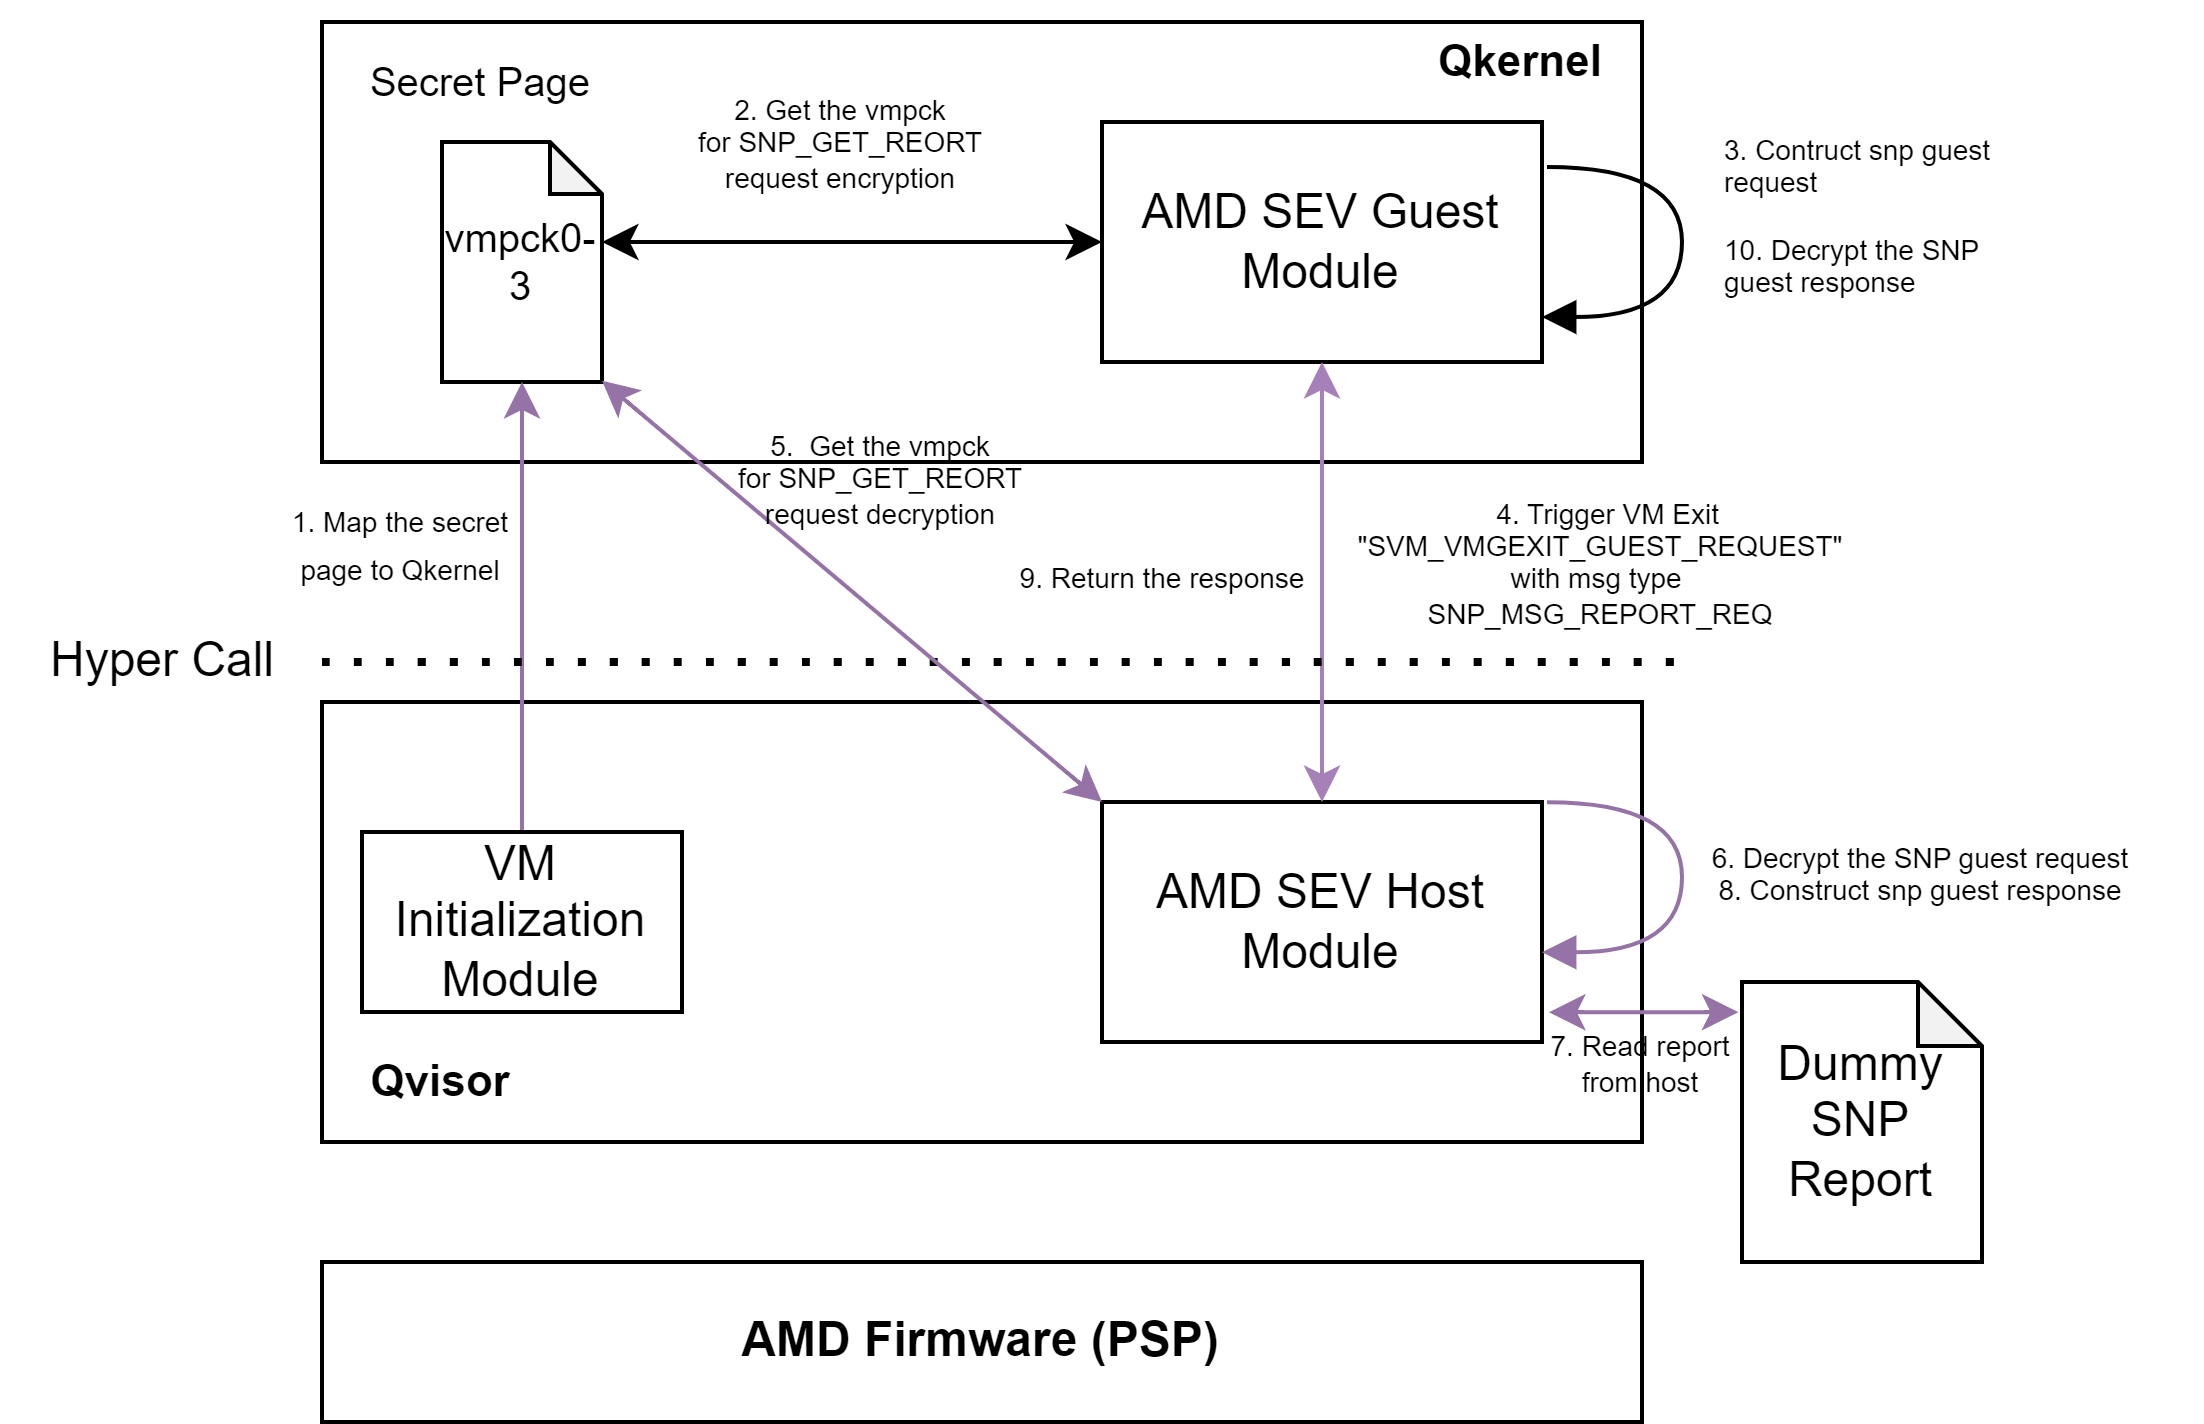
\includegraphics[width=0.8\textwidth]{images/amd_snp_driver.png}
    \caption[Attestation Driver Workflow]{Attestation Driver Workflow}
    \label{fig:amd_snp_driver}
\end{figure}

To simulate the aforementioned process, as shown in Figure~\ref{fig:amd_snp_driver}, Qvisor's VM initialization module initializes a secret page during the virtual machine's creation process. This page is mapped to shared memory between Qvisor and Qkernel. When the enclave requests an attestation 
report, the attestation driver creates an  SNP request using a VMPCK on the secret page. This request is relayed to the AMD SEV SNP firmware emulation module in Qvisor via the hyper call SVM\_VMGEXIT\_GUEST\_REQUEST. This module is responsible for emulating SNP firmware. It will decrypt the request 
using the vmpck on the page. A dummy report is then retrieved from the disk and tweaked according to the attestation driver's requirements for user-defined fields. Subsequently, the SNP module encrypts the altered report with vmpck and returns it to the attestation driver as the SNP response payload. The attestation driver can 
decrypt the response and retrieve the report using VMPCK.

This driver provides the API in Listing~\ref{lst:Attestation_driver} . It takes user-defined data and returns a report serialized as a JSON string. The user-defined data is added to the custom field of the report. Returning a string instead of a specific report allows extending this driver to support multiple TEEs. Specifically,  
When it receives a request to generate a report, it will generate a report in different formats depending on the type of TEE. Then, it will serialize this report into a string and return it to the requestor. The requestor can deserialize this string to get the specific report according to the TEE type
\begin{lstlisting}[language=rust, caption= API of attestation driver, label={lst:Attestation_driver}]
pub fn get_report(&mut self, report_data: String) -> Result<String>   
\end{lstlisting}

\subsection{Runtime Attestation Service}
The API of runtime attestation service is shown in the Listing~\ref{lst:runtime_attestation}. We have added a new system call with id 451 to the Qkernel. the SysAttestationReport function is the handler for this system call. It accepts user-defined data, data length, a structure called Request, and returns a report to 
the application. Here, the Request allows the application to specify the desired report type.

\begin{lstlisting}[language=rust, caption= Interface for accessing the file type secrets, label={lst:runtime_attestation}]

pub struct Requst {
    pub software_based_report_requered: bool,
    pub use_user_provided_signing_key: bool,
    pub signing_key_length: usize, 
    pub signing_Key: [u8; 4096],  
}

pub struct Report {
    //  AMD SNP: 2, TDX: 3, Software based: 4
    pub tee_type: u64,
    pub report_length: u64,
    //  AMD SNP REPORT has 1183 bytes, INTEL TDX report has 1024 bytes
    pub report: [u8; 4096],  
}

pub fn SysAttestationReport(task: &mut Task, args: &SyscallArguments) -> Result<i64>      
\end{lstlisting}

SysAttestationReport can generate software or hardware reports. To return a report of any type, the function serializes a report as a JSON string. It then converts the string into a byte array and embeds the array in the report field of the Report structure. After that, SysAttestationReport copies 
the Report structure to the address specified by the application. The application can get the length of the report character array from the report\_length in the Report structure. After converting the report character array to a string, the type of the report can be determined from the tee\_type field, 
and the string can then be deserialized to an appropriate report. The format of the software report has been described in the design chapter, while the format of a hardware report depends on the TEE type.

\section{Software measurement manager}
This section describes how software measurement managers measure data loaded from the host, e.g., dynamic libraries, binaries, etc., and how to get the four hash values described in the.
\todo{Add link}

\subsection{Binary Measurement}

\begin{figure}[!htb]
    \centering
    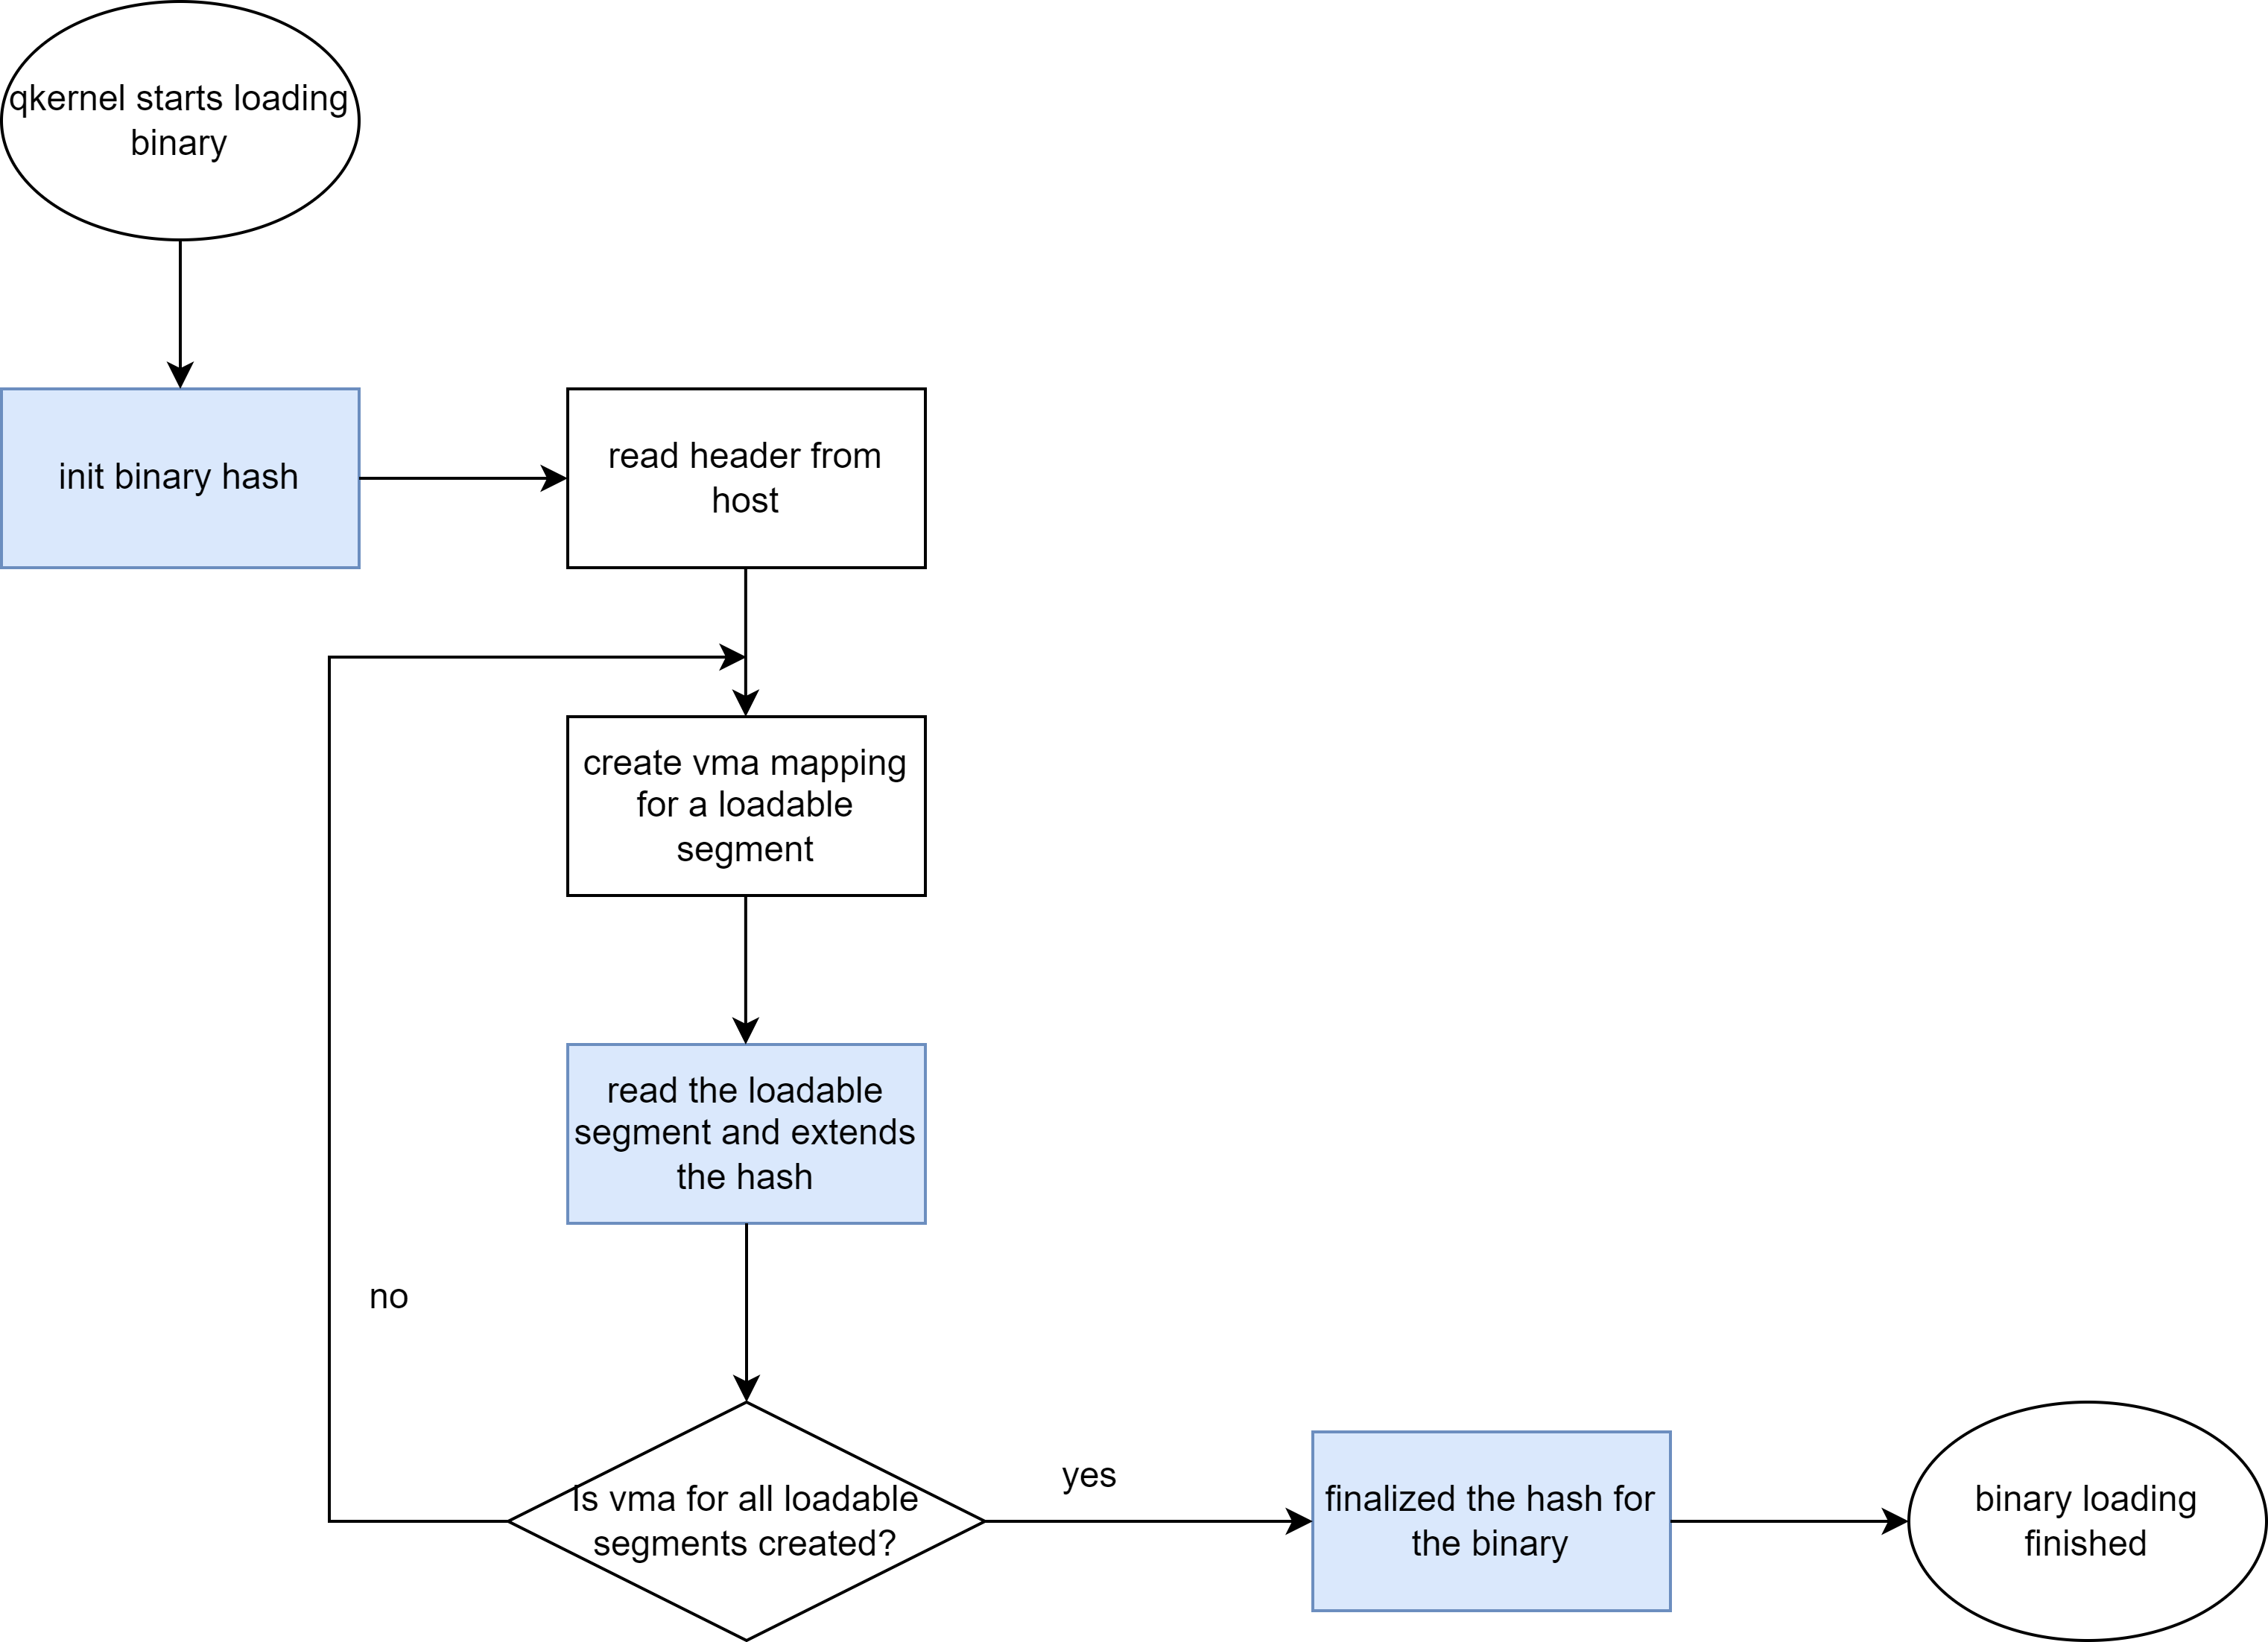
\includegraphics[width=0.8\textwidth]{images/measure_binary.png}
    \caption[Binary measurement workflow]{Binary measurement workflow}
    \label{fig:binary_measurement}
\end{figure}


The Figure~\ref{fig:binary_measurement} depicts the workflow of binary measurement. When the Qkernel loader starts loading a binary, the software measurement manager initializes a hash for it. The hash is then stored within a map. The secret manager can find the corresponding hash based on the name of the binary in the map. 
Subsequently, the loader reads the binary header and creates a Virtual Memory Area (VMA) for each loadable segment. Meanwhile, the software measurement manager reads the guest virtual address range of each VMA and extends the binary's hash utilizing the data read.
The read operation will trigger page fault handling, loading the corresponding data into the guest memory and setting up the page table. After the loader completes the creation of VMAs for all loadable segments, the software measurement manager obtains the binary measurement. Depending on the time the 
binary is loaded, the software measurement manager will process it differently. If the binary is loaded during application run-time, the resulting measurement will be compared with the reference value within the enclave policy. If the binary is loaded before the application process is launched, this 
measurement will extend the enclave startup measurement. If this measurement is loaded when restarting the application, it will extend the measurement associated with the application restart.

\subsection{Shared Library Measurement}

The workflow for shared library measurement is depicted in Figure~\ref{fig:measure_load_shared_libarart}. When the interpreter begins to load a dynamic library, it initiates the open system call to obtain the file descriptor for the shared library file. The open system call is processed by the Qkernel open system call handler。 
The handler determines whether a file is a shared library by checking its suffix (i.e., .so). If so, the handler notifies the secret manager to initialize a hash for the shared library, which is then stored in a B-tree map. Based on the library's name, the software manager can retrieve and extend the 
hash from the map.

\begin{figure}[!htb]
    \centering
    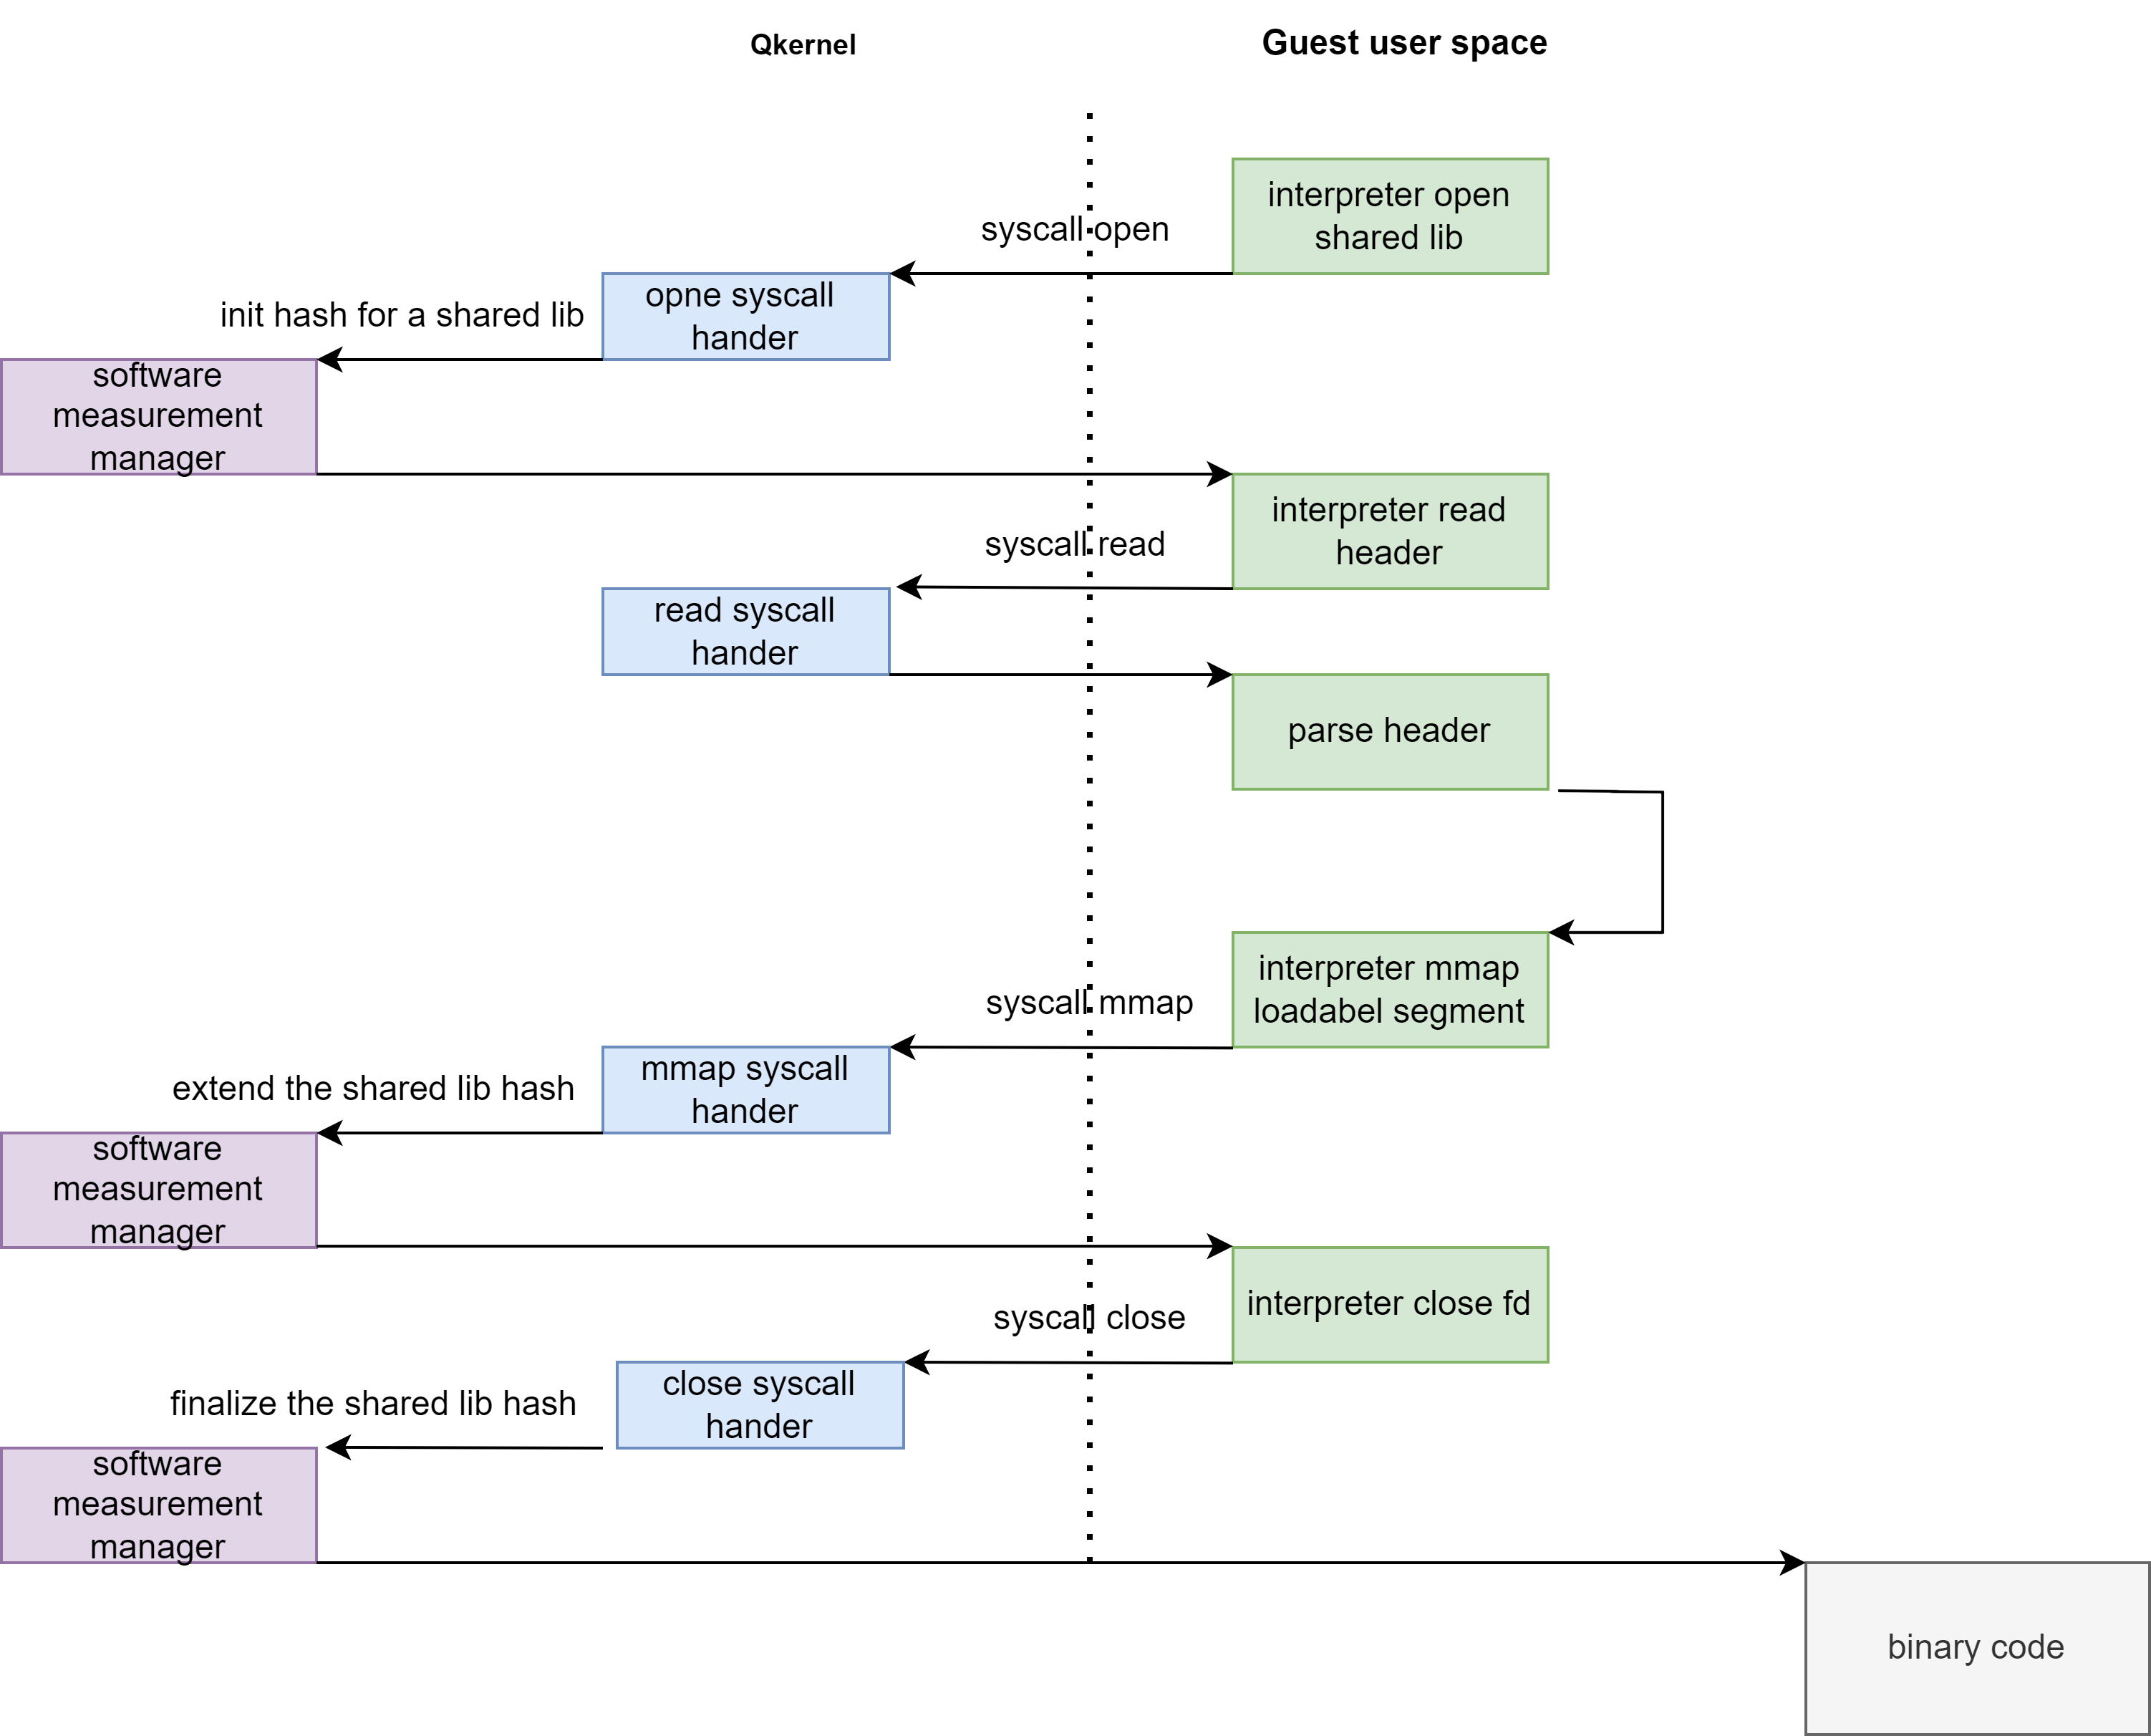
\includegraphics[width=0.8\textwidth]{images/measure_load_shared_libarart.png}
    \caption[Shared library measurement workflow]{Shared library measurement workflow}
    \label{fig:measure_load_shared_libarart}
\end{figure}


Once the open system call completes, the interpreter uses the read system call to read the library's header and find the loadable segments of the library. It then calls the mmap system call to create a virtual memory area (VMA) for each segment. After the Qkernel mmap system call handler creates a 
VMA,  the handler invokes the software measurement manager to measure it. Specifically, the manager reads the guest virtual memory range of the VMA and extends the library's hash using the data it reads. The read operation will cause the page fault handler to load the necessary data into the Qkernel. 
Since a shared library can have several shared segments, the mmap system call can be invoked several times. The library's hash may thus be extended multiple times.

Measuring the loadable segments of a shared library can be challenging. Since the shared library is location-independent, the interpreter may map it to any location supported by the Qkernel. The only requirement is that the Qkernel must make room for all the segments in their specified positions 
relative to the first segment. For this reason, the interpreter increases the mapping length to cover all the segments while mapping the first loadable segment. Since the mapping for all the segments might not be contiguous, the first VMA's virtual address range may be larger than the file size. 
This makes measuring the first segment difficult. If the software measurement manager reads the first VMA's address range directly, it may trigger a KVM segment fault. 

To avoid this,  as shown in Listing~\ref{lst:shared_Lib_measurement}, function measure\_shared\_lib\_loadable\_segment checks whether the mmmap\_len exceeds the size of the loadable file. If the mmmap\_len is larger, the interpreter maps the shared library's first loadable segment. By 
setting the real\_mmap\_size to the library's file size,measure\_shared\_lib\_loadable\_segment will measure the entire shared library. This enables the function to gauge the shared library's first segment and eliminate the possibility of a segment fault.

\begin{lstlisting}[language=rust, caption= Interface for accessing the file type secrets, label={lst:shared_Lib_measurement}]
pub fn measure_shared_lib_loadable_segment(&mut self, start_addr: u64, file: &File, task: &Task, fixed: bool, mmmap_len: u64, offset: u64, file_name: String) -> Result<()> {
    let uattr = file.UnstableAttr(task)?;
    let real_mmap_size = if uattr.Size as u64 > mmmap_len {
        mmmap_len
    } else {
        uattr.Size as u64
    };
    
    //read the range of the VMA
    let data: Result<Vec<u8>> = task.CopyInVec(start_addr, real_mmap_size as usize);
    ....
}
\end{lstlisting}
After creating the last VMA, the interpreter executes the close system call to release the shared library's file descriptor. The system call handler, in turn, notifies the software measurement manager that the library loading is completed. The software measurement manager then obtains the measurement 
result of the shared library from the map. Depending on the library's loading timing, the software measurement manager processes the result differently. When the shared library is loaded during the application's runtime, the software measurement manager compares the measurement result with the 
reference values in the enclave policy. Alternatively, if the library is loaded before the application process starts, the measurement will be used to extend the enclave startup measurement. Should this measurement occur upon application restart, it is saved and employed for comparison with the 
measurement during application startup. This approach ensures correct shared library is loaded during application restarts.

\subsection{Other Measurements}
Software measurement manager uses the SHA-512 hash function. This function accepts an array of bytes and returns a hash. Since the Qkernel configuration file is a structure, the software manager first serializes it into a JSON string and then converts it into a byte array. The generated array will 
be used as input to the hash function to extend the enclave startup measurement. The secret manager's public key is a byte array. After the software measurement manager reads it into the enclave from the directory /usr/local/secret\_manager\_cert.pem, it can be used directly to extend the enclave 
startup measurement.

\subsection{Implementation Detail}
The data structure presented in Listing~\ref{lst:shared_Lib_measurement_implementation_detail} maintained the metadata for the software measurement manager. The variables is\_app\_loaded, load\_app\_start, and load\_app\_end are employed to track the periods during which measurements are taken. 
The software measurement manager can decide what to do with the measurements based on these three variables. The variable runtime\_binary\_reference\_measurement stores the reference measurements for the binaries and shared libraries loaded at runtime. By utilizing these reference values, the software 
measurement manager can verify the integrity of these binaries and shared libraries. Variable global\_measurement is a hash, which can be used to track the measurement of binaries loaded after the enclave starts, the Qkernel configuration file, and secret manager’s public key.
Additionally, during program startup and restart, the software manager utilizes the variables app\_binary\_ref\_measurement and restart\_binary\_measurement to track the measurement of binaries. Moreover, the variable shared\_lib\_measurements and binary\_measurement record the temporary hash values 
assigned to shared libraries and binarise during the measurement process, respectively. The software manager can retrieve the corresponding hash by the file name and extend it accordingly.


\begin{lstlisting}[language=rust, caption= Interface for accessing the file type secrets, label={lst:shared_Lib_measurement_implementation_detail}]
pub struct SoftwareMeasurementManager {
    enclave_mode: EnclaveMode,
    is_app_loaded: bool,
    load_app_start: bool,
    load_app_end: bool,
    runtime_binary_reference_measurement:  BTreeMap<String, String>,
    global_measurement : String,
    enclave_ref_measurement: String,
    shared_lib_measurements: BTreeMap<String, String>,
    binary_measurement:  BTreeMap<String, String>,
    app_binary_ref_measurement : String,
    restart_bianry_measurement : String,
    startup_shared_lib_measurement_results:  BTreeMap<String, String>,
    restart_shared_lib_measurement_results:  BTreeMap<String, String>,
}
\end{lstlisting}

Since the order in which shared libraries are loaded may vary each time the application starts, software managers use BTreeMap to record the measurement results for each shared library during application startup and restart, i.e., startup\_shared\_lib\_measurement\_results and restart\_shared\_lib.
Each shared library has an entry in the BTreeMap. As the Qkernel might initiate multiple processes during application startup to establish the application environment, a shared library can be loaded and measured multiple times. Thus, when a shared library undergoes repeated measurement, 
the software manager compares the measurements stored in the BTreeMap with the hash obtained from the library's repeated measurement. If discrepancies arise between the two, the software manager triggers a panic.


Following the completion of the initial application setup, the software manager generates the enclave startup measurement using the measurements stored in global\_measurement and startup\_shared\_lib\_measurement\_results. This hash is then stored in the variable enclave\_ref\_measurement. The ordered 
nature of the BTreeMap ensures that the generated enclave startup hash remains consistent. 

The application startup reference measurement generally refers to the measurements stored in variable app\_binary\_ref\_measurement and startup\_shared\_lib\_measurement\_results, whereas the application restart measurements pertain to measurement in variable restart\_binary\_measurement and 
restart\_shared\_lib\_measurement\_results. When the application is restarted, the software measurement manager first compares the app\_binary\_ref\_measurement with the restart\_binary\_measurement. This guarantees that the binaries loaded during the application restart and initial startup are 
identical. Subsequently, a comparison is made between the measurements stored in startup\_shared\_lib\_measurement\_results and restart\_shared\_lib\_measurement\_results for the shared libraries. This verification ensures that all shared libraries loaded during application restart are consistent 
with those loaded during the initial application startup.

\section{EXEC Checker}
The Exec checker provides the Quark agent with the API shown in Listing~\ref{lst:exec_Cheker}. This function checks EXEC requests for legitimacy and handles session allocation or  policy update request from privileged users. It returns true if the EXEC request is legitimate and false if not. 
The execAuthenAcCheckArgs contains the metadata required to create an EXEC process. In particular, args is an array of strings containing the command to be executed and its arguments. 

\begin{lstlisting}[language=rust, caption= API of EXEC checker, label={lst:exec_Cheker}]
pub struct ExecAuthenAcCheckArgs {
    pub exec_id: String,
    pub args: Vec<String>,
    pub env: Vec<String>,
    pub cwd: String,
    pub req_type: ExecRequestType,
}
pub fn exec_req_authentication (exec_req: ExecAuthenAcCheckArgs) -> bool
\end{lstlisting}

The workflow of the function is illustrated in Figure~\ref{fig:exec_req_authentication_flow_chart}. Initially, it determines the privilege level of the request by examining whether the first element of the array matches the keyword "Privileged." If it does, the function validates and decrypts the 
encrypted payload in the array. Subsequently, it verifies the legitimacy of the request's session and counters. If these components are deemed illegitimate, the function returns false. It then identifies whether the request is a session assignment or policy update request using the methods described 
in Section~\ref{subsec:design_policy_session_update}. In the case of a typical Linux command, the function checks its legality based on the policy. Specifically, it first confirms if the command is included in the command allowlist. If it is, the function checks if the directory allowlist incorporates the path-like string found in the 
command's arguments. Notably, for a no-arguments command, the function verifies if the current execution directory of the command is present in the directory allowlist. For non-privileged commands, the function only evaluates their legality based on the policy. If a command meets the policy criteria, 
the function saves the EXEC request's command and argument in plaintext. The Quark agent can then employ the EXEC ID to retrieve a legitimate EXEC request's metadata and create the corresponding process.

\begin{figure}[!htb]
    \centering
    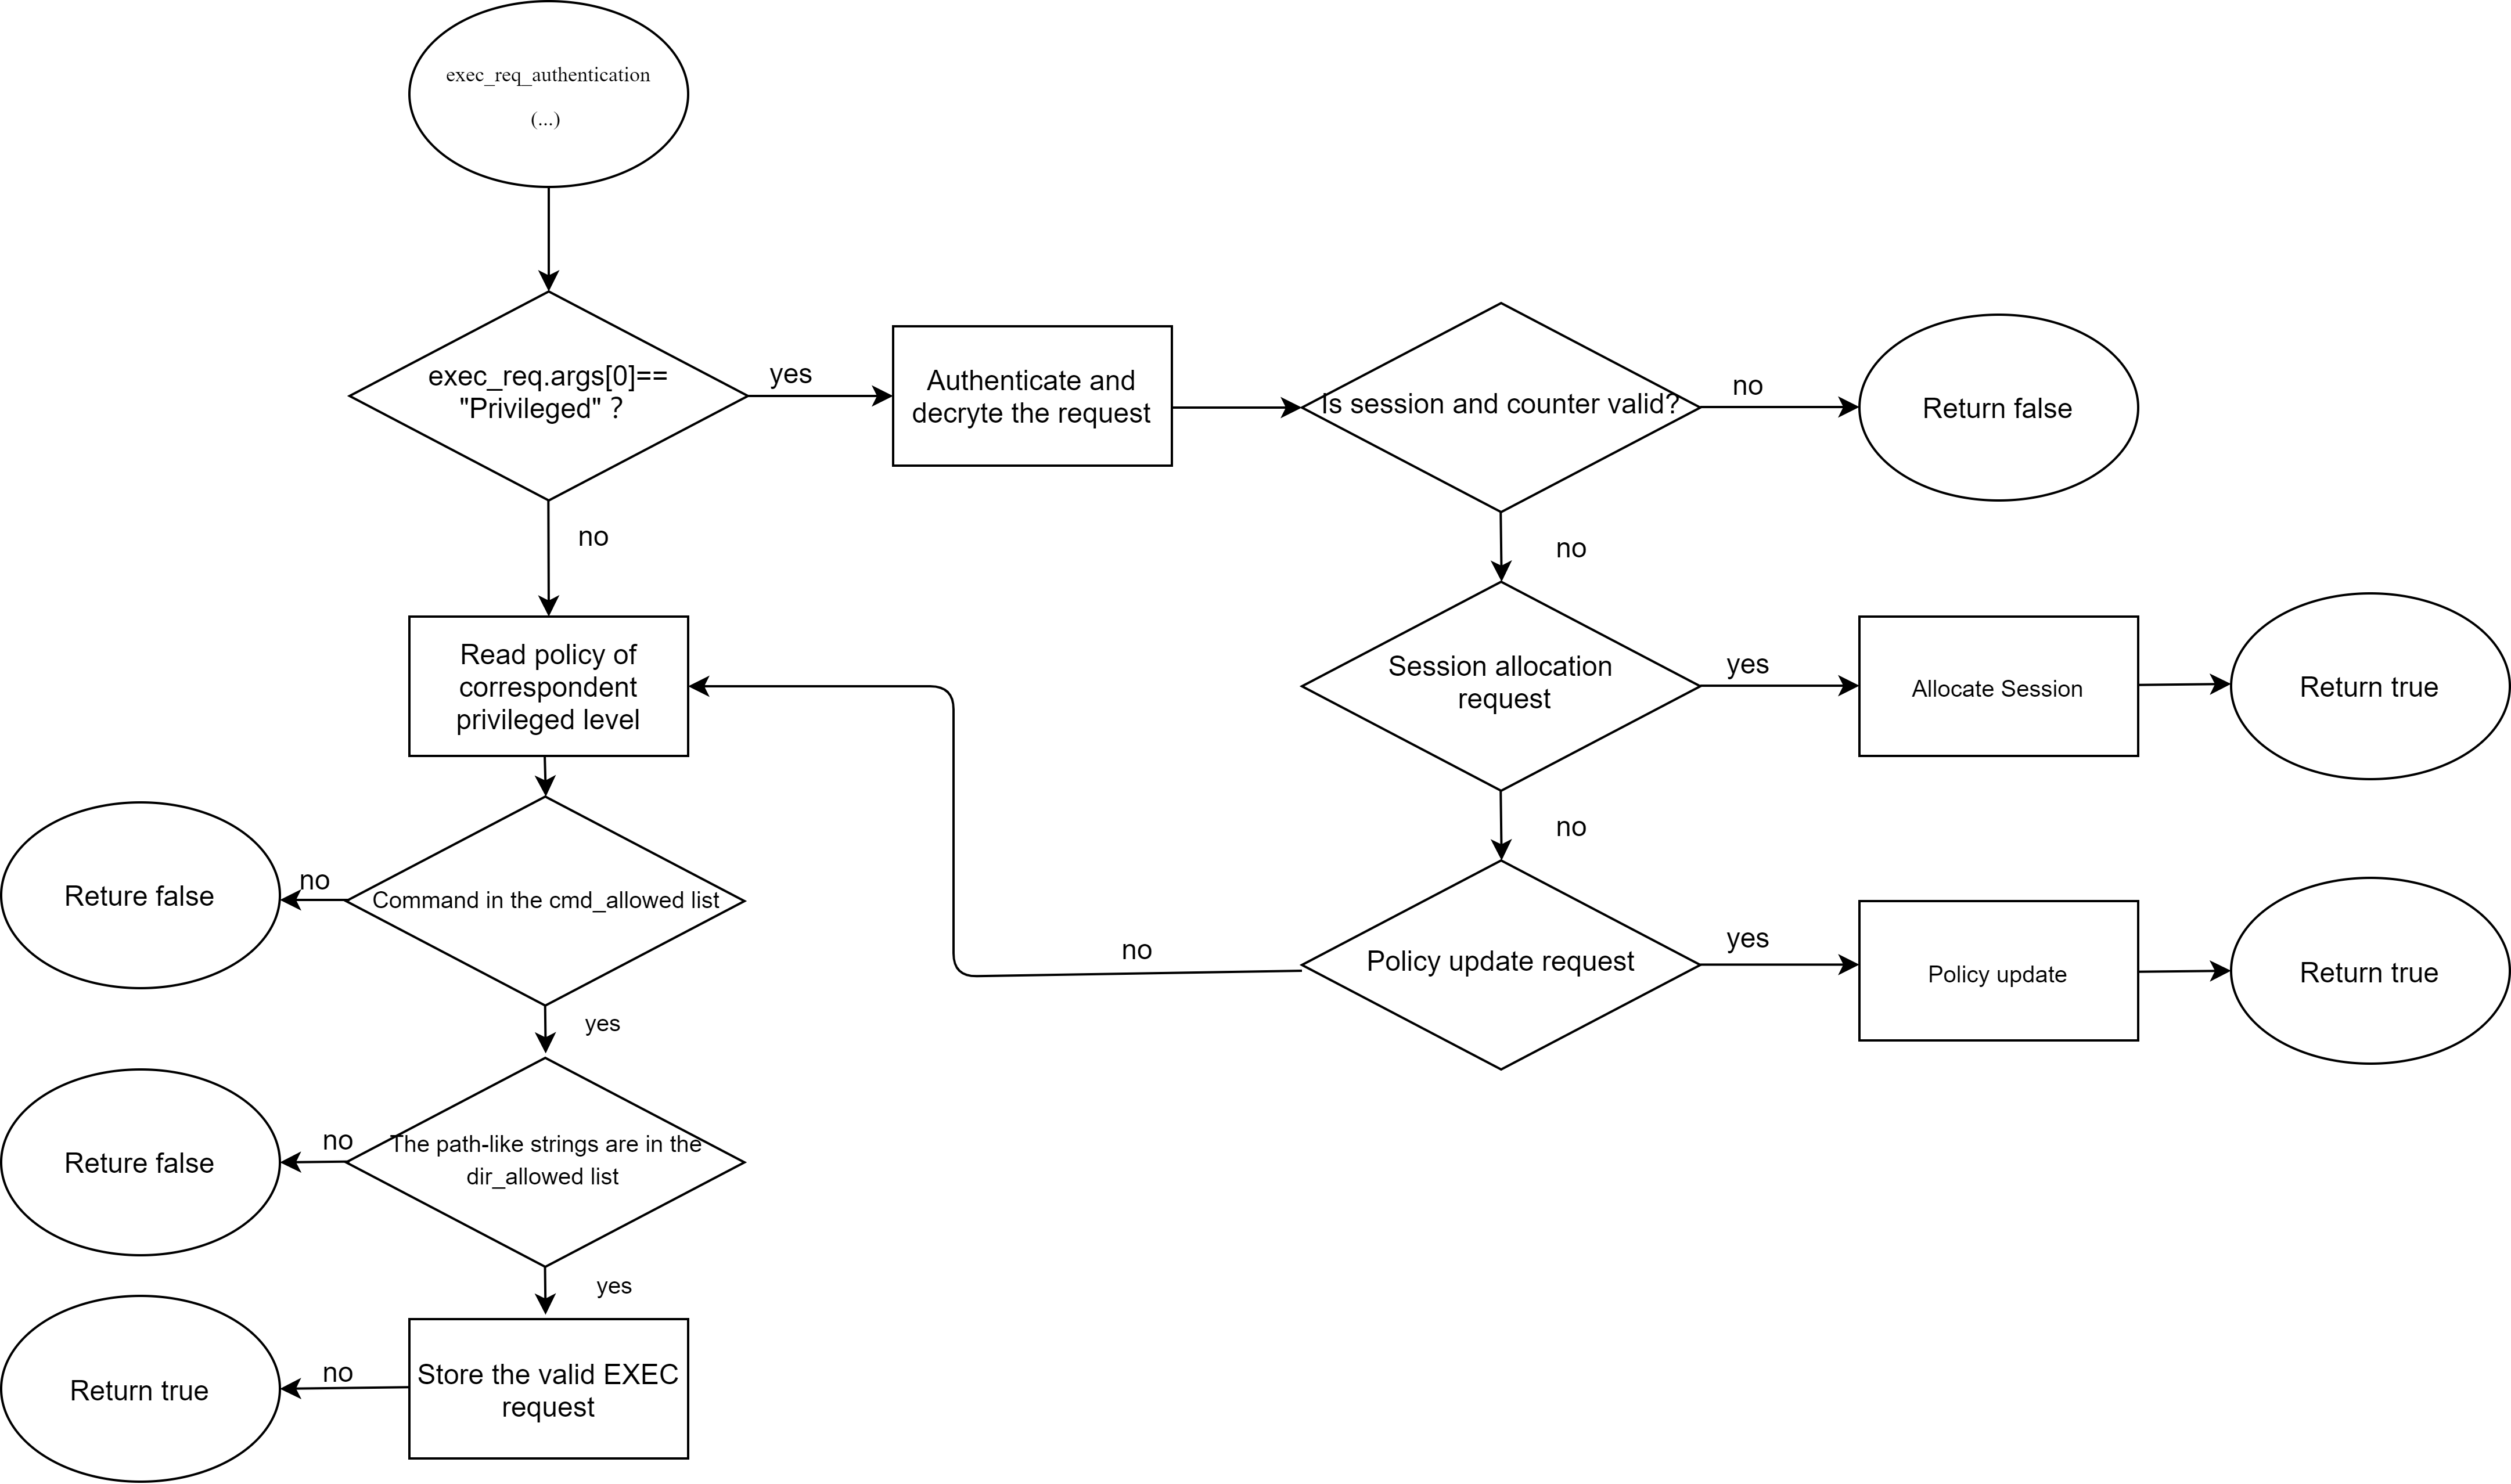
\includegraphics[width=0.8\textwidth]{images/exec_req_authentication_flow_chart.png}
    \caption[EXEC cheker workflow]{EXEC cheker workflow}
    \label{fig:exec_req_authentication_flow_chart}
\end{figure}

\section{STDIO Protection}

\subsection{Inode Tracker}
The data structure InodeTracker in Listing~\ref{lst:Inode_Tracker} records information about the file descriptor that is the process’s STDIO. It maintains a map where the key is the inode id, and the value contains the type of the file descriptor and some metadata. 
The detail of the data structure can be found in Section XX. For example, when the inode type is session, the metadata includes the session id and the counter assigned to a privileged user. Normal IO shield can take the session's metadata from the inode\_track, encrypt it, and send it to
the privileged user via STDOUT of an EXEC process.
\todo{e can be found in Section XX.}
\begin{lstlisting}[language=rust, caption= API of Inode Tracker, label={lst:Inode_Tracker}]
pub struct InodeTracker {
    inode_track: BTreeMap<u64, TrackInodeType>,
} 
\end{lstlisting}

\subsection{Normal IO Protection}
\begin{lstlisting}[language=rust, caption= API of normal IO shield, label={lst:Normal_IO}]
fn encrypNormalIOStdouterr (&self, src: DataBuff, inode_id: u64) -> Result<DataBuff>
\end{lstlisting}
The function in Listing~\ref{lst:Normal_IO} encrypts STDOUT and STDERR for processes whose STDIO type is Normal IO. It accepts the data written to STDOUT or STDERR and the id of the inode corresponding to the STDOUT or STDERR file descriptor. Depending on the enclave policy and inode type, the 
function encrypts the data using the method specified in section XX. Subsequently, it returns the encrypted data to Qkernel. Qkernel then sends encrypted data out via Qcall.


\subsection{Terminal IO Protection}
\begin{lstlisting}[language=rust, caption= API of system call interceptor, label={lst:Termianl_IO}]
fn termianlIoEncryption(&self, src: &[IoVec], task: &Task,  inode_id: u64) -> Result<(Vec::<IoVec>)
\end{lstlisting}
Like the encrypNormalIOStdouterr function, the function in Listing~\ref{lst:Termianl_IO} is responsible for encrypting the STDOUT and STDERR of processes whose STDIO is of terminal type. This not only ensures that the logs of the interactive application are encrypted but also prevents malicious 
users from attaching to the application.

\section{System Call Interceptor}
The three functions in the Listing~\ref{lst:Interceptor} are responsible for updating the interceptor’s policy at runtime, initializing the interceptor’s policy at enclave startup, and determining whether a system call is allowed. When the interceptor operates in ContextBased mode, 
the is\_guest\_syscall\_allowed function utilizes the application process id stored in the structure GuestSyscallInterceptor to identify whether a process is the application process. To prevent competition between the three functions accessing the interceptor's policy, the interceptor is 
protected by RwLock. Additionally, the BackEndSyscallInterceptorConfig maintains a vector that contains the id of allowed system calls (allowlist). The is\_guest\_syscall\_allowed function checks whether a system call's ID is present in this list to determine whether the system call is allowed. 
It is important to note that accessing this allowlist has an O(n) time complexity.

\begin{lstlisting}[language=rust, caption= API of system call interceptor, label={lst:Interceptor}]
static ref SYSCALLINTERCEPTOR:  RwLock<GuestSyscallInterceptor> = RwLock::new(GuestSyscallInterceptor::default());

pub struct BackEndSyscallInterceptorConfig {
    pub syscalls: Vec<u64>
…
}

pub struct GuestSyscallInterceptor {
    policy: BackEndSyscallInterceptorConfig,
    application_pid: i32,
}

pub fn syscall_interceptor_policy_update(policy: &BackEndSyscallInterceptorConfig) -> Result<()> 
pub fn syscall_interceptor_init(policy: BackEndSyscallInterceptorConfig) -> Result<()> 
pub fn is_guest_syscall_allowed(current_pid: i32, syscall_id: u64) -> bool
    
\end{lstlisting}


\section{Qlog Manager}

Listing~\ref{lst:Qlog} presents the API of the Qkernel log manager. The QlogManager structure maintains the Qlog manager's policy, as shown in Figure XX. The shielding layer uses the function  qlog\_manager\_init to initialize or update the policy. The function is\_log\_level\_allowed  is invoked by 
the Qkernel logging system. It accepts the level of the log that currently needs to be printed. It returns true if the log level is the same or less than the log level specified in the policy. If this function returns false, the Qkernel logging system will not print the log message.

\todo{icy, as shown in Figure XX}
\begin{lstlisting}[language=rust, caption= API of Qlog manager, label={lst:Qlog}]
pub struct QlogManager {
    policy: QlogPolicy,
}
pub fn is_log_level_allowed(current_log_level: QkernelDebugLevel) -> bool
pub fn qlog_magager_init()   
\end{lstlisting}


\section{Summary}
In this chapter, we explain how the design in Chapter~\ref{sec:design} was implemented. In the next chapter, we evaluate the performance and security of the system.


\cleardoublepage



%%% Local Variables:
%%% TeX-master: "diplom"
%%% End:

